\documentclass[11pt]{article}
\usepackage[T1]{fontenc}
\usepackage[utf8]{inputenc}
\usepackage[french]{babel}
\usepackage[a4paper,margin=2.2cm]{geometry}
\usepackage{amsmath,amssymb,graphicx,booktabs,hyperref,xcolor,enumitem}
\graphicspath{{../figures/}}
\setlist{itemsep=2pt,topsep=4pt}
\newcommand{\Mpch}{\,h^{-1}\mathrm{Mpc}}
\newcommand{\encadre}[1]{\par\smallskip\noindent\fcolorbox{gray!60}{gray!8}{\parbox{0.96\linewidth}{#1}}\par\smallskip}

\title{ASTRA, density split et cosmologie :\\ le projet expliqué simplement}
\author{Hugo Nguyen}
\date{}

\begin{document}
\maketitle

\noindent Ce document accompagne l'article. Il explique, sans prérequis, les notions utilisées, les choix faits et les questions qu'on peut se poser en le lisant. Les sections peuvent se lire dans le désordre.

\tableofcontents

% ======================================================================
\section{Le projet en quelques phrases}

\encadre{\textbf{Pourquoi.} La façon dont les galaxies sont réparties dans l'Univers dépend de quelques grandeurs fondamentales : la quantité de matière, l'amplitude des fluctuations, la nature de l'énergie noire, la masse des neutrinos. La statistique habituelle, la fonction de corrélation à deux points, ne capte qu'une partie de cette information, parce que la toile cosmique (amas, filaments, feuillets, vides) n'est pas un champ gaussien.

\textbf{Quoi.} On teste si ASTRA, un algorithme qui attribue un environnement à chaque point à partir de ses voisins, permet de récupérer cette information manquante, et s'il fait mieux ou moins bien que la méthode de référence, le \emph{density split}.

\textbf{Comment.} (1) On classe les galaxies et des points aléatoires par environnement, avec ASTRA et avec le density split. (2) On mesure comment ces environnements se regroupent (corrélations). (3) On estime, à l'aide de simulations, combien ces mesures varient quand on change les paramètres cosmologiques (dérivées) et combien elles fluctuent par hasard (covariance). (4) On en déduit les incertitudes attendues sur chaque paramètre (matrice de Fisher). (5) On vérifie toute la chaîne avec un émulateur par réseau de neurones et une inférence MCMC.

\textbf{Conclusion.} Les statistiques d'environnement ASTRA contraignent les paramètres environ deux fois mieux que la fonction à deux points. Elles sont aussi informatives que le density split et complémentaires : les combiner fait encore mieux. Les classes d'origine d'ASTRA (vides, feuillets, filaments, nœuds) donnent, sur les simulations Quijote, une contrainte sur $\sigma_8$ deux à trois fois meilleure que le density split.}

\paragraph{La chaîne d'analyse (pipeline).}
\begin{center}
\small
catalogues de galaxies $\to$ environnements (ASTRA, density split) $\to$ quartiles / classes $\to$ corrélations (monopôle, quadrupôle) $\to$ covariance + dérivées $\to$ matrice de Fisher $\to$ incertitudes sur les paramètres $\to$ comparaison 2PCF / density split / ASTRA
\end{center}

% ======================================================================
\section{Les bases de cosmologie}

\subsection{Le redshift}
La lumière d'une galaxie lointaine nous arrive « étirée » vers le rouge, parce que l'Univers s'est dilaté pendant son trajet. Ce décalage, le \emph{redshift} $z$, mesure donc à la fois la distance et l'époque : $z=0.5$ correspond à une lumière émise il y a environ 5 milliards d'années. Les relevés comme DESI mesurent le redshift de chaque galaxie pour la placer en 3D.

\paragraph{Les distorsions dans l'espace des redshifts (RSD).} Une galaxie ne fait pas que suivre l'expansion : elle bouge aussi, attirée par les structures voisines. Cette vitesse propre ajoute un petit décalage Doppler, si bien que la position déduite du redshift est légèrement fausse le long de la ligne de visée. Autour d'un amas, les galaxies qui tombent vers lui semblent écrasées le long de la ligne de visée ; autour d'un vide, les galaxies qui s'en éloignent semblent étirées. Ces distorsions sont une nuisance mais aussi une information : elles mesurent la vitesse de croissance des structures.

\subsection{Les paramètres que l'on veut contraindre}
Le modèle standard, $\Lambda$CDM, décrit l'Univers avec une poignée de paramètres :
\begin{itemize}
\item $\omega_b$ et $\omega_{\rm cdm}$ : la densité de matière ordinaire (baryons) et de matière noire froide. Leur somme donne $\Omega_m$, la fraction de l'Univers faite de matière. Elles fixent la vitesse à laquelle les structures se forment et la forme de la fonction de corrélation.
\item $\sigma_8$ : l'amplitude des fluctuations de densité aujourd'hui (sur des sphères de $8\Mpch$). Plus $\sigma_8$ est grand, plus l'Univers est « grumeleux ».
\item $n_s$ : la manière dont l'amplitude des fluctuations initiales dépend de l'échelle (héritée de l'inflation).
\item $h$ : le taux d'expansion actuel (constante de Hubble). Dans AbacusSummit il est fixé par les autres paramètres.
\item $\alpha_s$, $N_{\rm ur}$ : des extensions (variation de $n_s$ avec l'échelle, nombre d'espèces relativistes).
\end{itemize}

\paragraph{L'énergie noire ($w_0$, $w_a$).} L'expansion de l'Univers accélère depuis quelques milliards d'années. On attribue cette accélération à une « énergie noire » dont on ignore la nature. Si c'est une constante cosmologique, sa pression vaut exactement $-1$ fois sa densité : $w=-1$. Les paramètres $w_0$ et $w_a$ décrivent un éventuel écart à cette valeur et son évolution dans le temps ($w = w_0 + w_a(1-a)$). Les premiers résultats de DESI suggèrent justement un tel écart : mieux contraindre $w_0$ et $w_a$ est l'un des enjeux majeurs actuels.

\paragraph{Les neutrinos ($\sum m_\nu$).} Les neutrinos sont des particules très légères dont on sait qu'elles ont une masse, mais pas laquelle. Leur somme des masses $\sum m_\nu$ est un paramètre de physique fondamentale que la cosmologie peut mesurer : des neutrinos massifs se déplacent vite et « lissent » les petites structures, ce qui freine leur croissance. Cet effet est subtil et apparaît surtout dans les environnements extrêmes (vides, amas) : c'est pour cela que les statistiques d'environnement sont prometteuses pour $\sum m_\nu$ (cf. Sunseri et al.).

\paragraph{Pourquoi et comment on les « contraint ».} Contraindre un paramètre, c'est réduire l'intervalle des valeurs compatibles avec les observations. On quantifie cela par l'incertitude $\sigma$ attendue sur le paramètre : une statistique est meilleure qu'une autre si elle donne un $\sigma$ plus petit avec les mêmes données. Dans l'article, on compare toujours des rapports d'incertitudes, par exemple $\sigma_{\rm 2PCF}/\sigma_{\rm ASTRA}=2$ veut dire qu'ASTRA réduit l'incertitude d'un facteur 2, ce qui équivaut à un relevé 4 fois plus grand.

% ======================================================================
\section{Les statistiques utilisées}

\subsection{La fonction de corrélation à deux points (2PCF)}
La 2PCF $\xi(s)$ mesure l'excès de paires de galaxies séparées d'une distance $s$ par rapport à une distribution au hasard. $\xi(s)>0$ : on trouve plus de paires que par hasard à cette distance, les galaxies sont regroupées. Son équivalent dans l'espace de Fourier est le spectre de puissance.

Dans la plupart des analyses, toute l'information cosmologique est comprimée dans ces statistiques à deux points. Elles sont optimales pour des champs gaussiens : un champ gaussien est entièrement décrit par sa moyenne et ses corrélations à deux points, il n'y a rien d'autre à mesurer. Aux grandes échelles, la distribution de matière reste proche d'un champ gaussien, et la 2PCF y est extrêmement performante.

\subsection{Pourquoi la 2PCF ne suffit pas}
La distribution de matière « tardive » (aujourd'hui) devient fortement non gaussienne. La gravité amplifie les surdensités : la matière s'effondre en halos, se rassemble dans des filaments et des nœuds, et vide les régions sous-denses. La distribution des densités devient très asymétrique (quelques amas très denses, beaucoup de vides). Les RSD ajoutent une autre déformation. Une partie de l'information se loge alors dans des corrélations à trois points, quatre points, etc., que la 2PCF ne voit pas.

On pourrait mesurer directement ces corrélations d'ordre supérieur (fonction à trois points, bispectre), mais elles sont coûteuses, bruitées et difficiles à modéliser. Les statistiques d'environnement sont une alternative : en séparant les régions denses et peu denses avant de mesurer des corrélations à deux points, on capte indirectement une partie de cette information d'ordre supérieur.

\subsection{Monopôle et quadrupôle}
À cause des RSD, la corrélation n'est pas la même le long de la ligne de visée et perpendiculairement. On mesure donc $\xi(s,\mu)$, où $\mu$ est le cosinus de l'angle entre la paire et la ligne de visée, et on le décompose en polynômes de Legendre :
\begin{itemize}
\item le \textbf{monopôle} $\xi_0(s)$ est la moyenne sur toutes les directions : l'amplitude du regroupement ;
\item le \textbf{quadrupôle} $\xi_2(s)$ mesure l'anisotropie, c'est-à-dire la différence entre le long et le travers de la ligne de visée : c'est la signature des vitesses (écrasement autour des amas : quadrupôle négatif ; étirement autour des vides : positif).
\end{itemize}
On multiplie par $s^2$ sur les figures ($s^2\xi$) uniquement pour rendre lisibles les grandes échelles.

\subsection{Auto-corrélations et corrélations croisées}
On découpe les points en environnements (par exemple Q1 = les plus sous-denses, Q4 = les plus denses). Pour chaque environnement :
\begin{itemize}
\item la \textbf{corrélation croisée} quartile--galaxies mesure combien de galaxies on trouve à une distance $s$ des points de ce quartile. Pour Q1, elle est négative à petite distance : c'est le \emph{profil} des galaxies autour d'un vide. Pour Q4, elle est forte et positive : le profil autour d'un amas.
\item l'\textbf{auto-corrélation} du quartile mesure comment les points du quartile se regroupent entre eux : comment les vides (ou les amas) sont répartis dans l'espace les uns par rapport aux autres.
\end{itemize}
Les deux portent des informations différentes : la première décrit la forme des structures, la seconde leur distribution à grande échelle. Dans nos résultats, l'auto-corrélation apporte un gain d'un facteur 1.3 à 2.8, et c'est elle qui donne l'avantage aux classes ASTRA sur $\sigma_8$.

\paragraph{Un quartile seul face à la 2PCF.} La 2PCF fait la moyenne du regroupement sur tous les environnements. Un quartile ne mesure que le regroupement autour d'une gamme de densités. Pour les quartiles de galaxies, la moyenne des quatre corrélations croisées redonne exactement la 2PCF : les quartiles « découpent » la 2PCF par environnement. Un quartile seul contient à peu près autant d'information que la 2PCF, mais pas la même ; c'est en les combinant, parce que les vides et les amas réagissent différemment à la cosmologie, qu'on gagne.

% ======================================================================
\section{Galaxies, halos et HOD}

\subsection{Les objets}
\begin{itemize}
\item \textbf{Particule} : dans une simulation $N$-corps, la matière (essentiellement noire) est représentée par des milliards de « particules » numériques, chacune pesant des milliards de masses solaires. Ce ne sont pas des particules physiques, mais des morceaux de fluide qui suivent la gravité.
\item \textbf{Halo} : un amas de particules lié par la gravité, le lieu où se forment les galaxies. On les repère dans la simulation avec un « halo finder » ; \textbf{Rockstar} est l'un d'eux (il regroupe les particules proches en position et en vitesse). Dans Quijote, on garde les halos d'au moins 100 particules.
\item \textbf{Galaxie} : les simulations de matière noire ne contiennent pas de galaxies. On les ajoute ensuite dans les halos avec un modèle statistique, la HOD.
\item \textbf{LRG} (Luminous Red Galaxies) : des galaxies massives, rouges et lumineuses, l'une des populations cibles de DESI. Elles vivent dans des halos massifs.
\item \textbf{Traceur} : tout ce qu'on utilise pour « tracer » la matière : galaxies, halos.
\item \textbf{Points aléatoires} : des points tirés uniformément dans la boîte, sans aucune structure. Ils servent de référence « sans regroupement », et de points de sondage pour décrire l'environnement partout, y compris dans les vides où il n'y a pas de galaxies.
\end{itemize}

\subsection{La HOD (Halo Occupation Distribution)}
La HOD est une recette qui dit combien de galaxies mettre dans un halo selon sa masse : en dessous d'une certaine masse aucune galaxie ; au-dessus une galaxie centrale, puis de plus en plus de galaxies satellites. Elle a ici 12 paramètres : la masse minimale, la pente du nombre de satellites, la dispersion, les vitesses des galaxies dans le halo, l'effet de l'environnement, etc. Ce ne sont pas des paramètres cosmologiques : ils décrivent la formation des galaxies, mal connue, et on doit les marginaliser (les laisser libres) pour ne pas biaiser la cosmologie.

\paragraph{« Un tirage de HOD indépendant par cosmologie ».} Les catalogues que nous avons utilisés ne sont pas des données réelles : ce sont des catalogues simulés (\emph{mocks}). Pour chaque cosmologie, on a pris une simulation de matière noire et on l'a peuplée de galaxies 500 fois, avec 500 jeux de paramètres HOD différents, tirés au hasard dans une plage (un « hypercube latin »). Ces 500 fichiers ne sont donc pas 500 réalisations du même modèle : ce sont 500 modèles de galaxies différents. Et le fichier \texttt{hod042} d'une cosmologie n'a pas les mêmes paramètres que le \texttt{hod042} d'une autre. C'est voulu : ces catalogues ont été produits pour entraîner un émulateur, qui doit voir beaucoup de combinaisons différentes.

\paragraph{Pourquoi plusieurs échantillons, si les galaxies sont « réelles » ?} Justement, elles ne le sont pas : dans l'Univers réel, il n'existe qu'un seul jeu de galaxies et une seule HOD (inconnue). Les simulations permettent d'essayer de nombreuses HOD possibles pour apprendre comment les statistiques en dépendent.

\paragraph{Si les paramètres HOD sont comme des hyperparamètres, pourquoi ne pas tout générer ?} En principe on pourrait générer, pour chaque cosmologie, des catalogues avec \emph{exactement} la même HOD : c'est ce qui donnerait les dérivées les plus propres. Deux obstacles : (1) il faut pour cela les sous-échantillons de particules préparés pour AbacusHOD dans chaque cosmologie, que nous n'avions pas (c'est une question pour Jaime) ; (2) chaque génération plus mesure coûte du temps de calcul. Nous avons donc travaillé avec les catalogues existants, et c'est ce qui a rendu les dérivées difficiles.

\paragraph{« La dispersion entre tirages de HOD atteint 55\% contre 1\% pour la cosmologie ».} Si l'on compare deux fichiers HOD d'une même cosmologie, leurs statistiques diffèrent en moyenne de 55\% de l'amplitude du signal, simplement parce que ce sont deux modèles de galaxies différents. Changer un paramètre cosmologique d'un petit pas, lui, ne change les statistiques que d'environ 1\%. Si l'on compare deux cosmologies avec des HOD différentes, l'effet HOD (55\%) noie complètement l'effet cosmologique (1\%). C'est tout le problème des dérivées.

\subsection{Cosmologie, phase, graine}
\begin{itemize}
\item \textbf{Cosmologie} : un jeu de paramètres cosmologiques (la suite en propose 85, notées \texttt{c000}, \texttt{c001}, etc. ; \texttt{c000} est la cosmologie de référence, Planck 2018).
\item \textbf{Phase} : les conditions initiales de la simulation, c'est-à-dire le tirage aléatoire des fluctuations primordiales. Deux simulations de même phase partent des « mêmes » fluctuations : elles forment les mêmes structures aux mêmes endroits, à la cosmologie près. Dans la suite d'émulation, toutes les cosmologies partagent la phase \texttt{ph000}.
\item \textbf{Graine (seed) de HOD} : la HOD est probabiliste (un halo a une certaine probabilité d'avoir une galaxie). La graine fixe ce tirage aléatoire. Une seule graine (\texttt{seed0}) existe ici.
\end{itemize}

% ======================================================================
\section{Les trois jeux de données}

\begin{center}\small
\begin{tabular}{p{3.2cm}p{4.8cm}p{6.5cm}}
\toprule
 & Contenu & Pourquoi on l'utilise \\
\midrule
AbacusSummit (suite d'émulation) & galaxies LRG simulées, 85 cosmologies, 500 HOD par cosmologie, 1 phase & le seul jeu avec beaucoup de cosmologies : mesures, entraînement de l'émulateur, dérivées type DESI \\
Mocks officiels DESI & mêmes simulations AbacusSummit, une seule cosmologie et une seule HOD (ajustée sur les vraies données DESI), mais 1786 petites boîtes indépendantes & beaucoup de réalisations indépendantes du même modèle : la covariance, et le point fiduciel \\
Quijote & simulations de matière noire, halos seulement (pas de galaxies), 500 paires $\pm$ par paramètre & dérivées « propres » sans problème de HOD \\
\bottomrule
\end{tabular}
\end{center}

\paragraph{Abacus et mocks officiels DESI : quelle différence ?} Les deux viennent des simulations AbacusSummit et de la même méthode (AbacusHOD). La suite d'émulation \emph{varie} la cosmologie et la HOD pour apprendre leurs effets, mais n'a qu'une réalisation par point. Les mocks officiels \emph{fixent} cosmologie et HOD (la meilleure HOD ajustée sur DESI) mais en ont 1786 réalisations indépendantes. L'un sert aux dérivées, l'autre à la covariance.

\paragraph{Comparer LRG et Quijote « sur les mêmes halos ».} Dans Quijote il n'y a pas de galaxies, donc on applique ASTRA et le density split directement aux halos. « Mêmes halos » signifie que les deux méthodes sont mesurées sur exactement le même catalogue de halos, donc la comparaison ASTRA/density split est équitable. En revanche, ces halos sont dix fois plus rares que nos LRG et ne sont pas des galaxies DESI : on ne compare pas les chiffres absolus entre Quijote et Abacus, seulement le classement des méthodes.

\paragraph{Pourquoi Quijote n'a pas de problème de HOD.} Les halos sont définis par la simulation elle-même (Rockstar les trouve), sans aucun modèle de galaxies. Quand on change la cosmologie, on compare les halos des deux simulations : rien d'autre ne change. Le prix à payer est le réalisme : des halos ne sont pas des LRG, donc Quijote sert de comparaison contrôlée des méthodes, complémentaire de l'analyse de type DESI.

\paragraph{Pourquoi des « particules de 100 » ?} Un halo de moins de 100 particules est mal résolu (on ne sait pas bien s'il existe). Ce seuil fixe la densité des halos de Quijote.

% ======================================================================
\section{La mesure}

\subsection{ASTRA}
On mélange les galaxies et autant de points aléatoires, et on calcule la triangulation de Delaunay de l'ensemble (on relie chaque point à ses voisins naturels). Pour chaque point, galaxie ou aléatoire, on compte ses voisins galaxies $N_{\rm data}$ et ses voisins aléatoires $N_{\rm rand}$, et on calcule $r=(N_{\rm data}-N_{\rm rand})/(N_{\rm data}+N_{\rm rand})$. \textbf{Oui, le $r$ des points aléatoires est calculé avec les galaxies et les autres points aléatoires} : c'est le même calcul pour tous. Un point entouré de galaxies est dans une région dense ($r\to1$), un point entouré de points aléatoires dans un vide ($r\to-1$).

\paragraph{L'extension de 30 Mpc/h.} On calcule ASTRA par sous-volume. Près des bords, un point a moins de voisins qu'il ne devrait, ce qui fausse $r$. On ajoute donc autour de chaque sous-volume une couche de $30\Mpch$ de points (en tenant compte de la périodicité de la boîte), qu'on n'utilise que comme voisins. La distance moyenne entre deux points voisins est d'environ $10\Mpch$ : la couche contient donc trois « rangées » de voisins, ce qui suffit (on l'a vérifié en passant à 60).

\subsection{Le density split}
On calcule une densité lissée : (1) on découpe la boîte en petits cubes de $5\Mpch$ et on compte les galaxies dans chaque cube. Le schéma « nuage dans la cellule » (CIC) répartit chaque galaxie entre les 8 cubes voisins au prorata de sa position, pour éviter des sauts brusques ; (2) on lisse ce champ avec une gaussienne de rayon $10\Mpch$, c'est-à-dire qu'on remplace la densité en chaque point par une moyenne pondérée sur une sphère d'environ $10\Mpch$. Ce n'est pas une dérivée : c'est une moyenne locale, qui définit « la densité de l'environnement à l'échelle de $10\Mpch$ » et supprime le bruit dû au nombre fini de galaxies. ASTRA, lui, n'a pas d'échelle fixe : il utilise les voisins, quelle que soit leur distance.

\subsection{Quartiles de points aléatoires et de galaxies}
On classe les points selon leur environnement et on les répartit en quatre groupes de même taille. On le fait séparément pour deux populations :
\begin{itemize}
\item \textbf{quartiles aléatoires} : les points aléatoires. Comme ils remplissent l'espace uniformément, chaque quartile représente un quart du \emph{volume} : Q1 = le quart du volume le plus vide. C'est la version standard du density split.
\item \textbf{quartiles de galaxies} : les galaxies elles-mêmes. Comme les galaxies sont concentrées dans les régions denses, chaque quartile représente un quart des galaxies, donc de la \emph{masse}.
\end{itemize}
On les classe séparément pour que les seuils d'une population ne dépendent pas de l'autre.

\subsection{Sous-volumes et estimateur de Landy--Szalay}
Chaque boîte de $2\,h^{-1}$Gpc est découpée en 64 sous-volumes de $500\Mpch$, chacun traité comme un petit relevé. Pour mesurer une corrélation, on compte les paires de points à chaque distance et on compare au nombre attendu sans regroupement. L'estimateur de Landy--Szalay fait cette comparaison avec un catalogue de points aléatoires « de géométrie » qui remplit le même volume :
$\xi=(DD-DR-RD+RR)/RR$. « Ouvert » veut dire qu'on traite le sous-volume comme une région isolée, avec des bords (comme un vrai relevé), et non comme une boîte périodique : les points aléatoires de géométrie corrigent l'effet des bords. On applique exactement la même méthode aux petites boîtes officielles, pour que la covariance corresponde à la même mesure.

\paragraph{« Une petite boîte périodique n'a pas de modes plus grands que son côté ».} Une simulation de $500\Mpch$ de côté ne contient aucune fluctuation plus grande que $500\Mpch$. Un sous-volume de $500\Mpch$ découpé dans une boîte de $2000\Mpch$, lui, baigne dans des fluctuations plus grandes (il peut être globalement un peu plus dense ou moins dense que la moyenne). Cela ajoute un peu de variance (« super-sample covariance »). L'effet est petit ici, et peut être mesuré avec les 25 grandes boîtes officielles.

% ======================================================================
\section{Covariance}

La covariance décrit combien une mesure fluctue par hasard, et comment ses différents bins fluctuent ensemble, à modèle fixé. C'est ce qui détermine les barres d'erreur.

\paragraph{Pourquoi 64 sous-volumes d'une même simulation donnent une covariance.} Même avec les mêmes paramètres, deux régions différentes de l'Univers ne contiennent pas les mêmes structures : c'est la « variance cosmique ». Les 64 sous-volumes d'une boîte sont 64 régions différentes, donc 64 échantillons de cette variance, à paramètres fixés : c'est exactement ce qu'on veut. Mais ils ont des défauts : ils viennent d'une seule boîte (ils partagent ses grandes fluctuations), et les trois lignes de visée réutilisent les mêmes galaxies. C'est pourquoi on a remplacé cette covariance par celle des 1786 boîtes officielles, qui sont vraiment indépendantes. Ce changement a d'ailleurs modifié le classement ASTRA / density split, ce qui montre son importance.

% ======================================================================
\section{Dérivées}

Pour savoir combien une mesure contraint un paramètre, il faut savoir de combien elle change quand le paramètre change : c'est la dérivée.

\paragraph{Différences finies.} La méthode la plus simple : simuler l'Univers avec le paramètre un peu plus grand ($+$) et un peu plus petit ($-$), et calculer (mesure$_+$ $-$ mesure$_-$)/(écart). Dans AbacusSummit, les fichiers $+$ et $-$ n'ont pas la même HOD : la différence mesure surtout le changement de HOD (10 fois plus grand que l'effet cosmologique). C'est le sens de la phrase « les différences finies entre cosmologies sont dominées par le changement de HOD ».

\paragraph{L'émulateur.} On entraîne un réseau de neurones qui prédit chaque statistique à partir des 8 paramètres cosmologiques et des 12 paramètres HOD, sur 999 catalogues. Une fois entraîné, on peut lui demander la dérivée par rapport à un paramètre cosmologique \emph{à HOD exactement fixée}, ce qui supprime le problème. On a vérifié ces dérivées par une méthode indépendante, une \textbf{régression} : dans chaque cosmologie $\pm$, on ajuste une droite des statistiques en fonction de la HOD, et on compare les deux cosmologies au même point HOD.

\paragraph{Différences centrales appariées (Quijote).} Dans Quijote, chaque simulation $+$ a une jumelle $-$ avec la même phase (mêmes conditions initiales). En faisant la différence jumelle par jumelle, la variance cosmique, commune aux deux, s'annule presque entièrement ; on moyenne ensuite sur les 500 paires. C'est beaucoup plus précis que de comparer des simulations indépendantes.

\paragraph{Le cas des neutrinos.} La masse des neutrinos ne peut pas être négative : on ne peut pas simuler un « $-$ » autour de $M_\nu=0$. On utilise donc une formule à trois points d'un seul côté, $(-3f_0+4f_{0.1}-f_{0.2})/0.2$, avec des simulations à $M_\nu=0$, $0.1$ et $0.2$ eV. Les simulations avec neutrinos de Quijote partent de conditions initiales calculées d'une façon particulière (approximation de Zel'dovich) ; pour que la comparaison soit propre, le point $M_\nu=0$ utilise des simulations fiducielles générées de la même façon (\texttt{fiducial\_ZA}).

\paragraph{Le bruit des dérivées.} Même appariées, les dérivées Quijote restent bruitées : peu de halos par quartile, et un petit changement de cosmologie fait passer des points d'un quartile à l'autre de façon un peu aléatoire. Ce bruit ajoute de la « fausse information », surtout pour les paramètres dégénérés ($\Omega_b$, $h$, $M_\nu$). On le détecte en comparant deux estimateurs de Fisher, l'un biaisé vers le haut et l'autre vers le bas : s'ils sont d'accord, le résultat est fiable.

\paragraph{Le prior.} Le prior est ce qu'on sait (ou suppose) d'un paramètre avant la mesure. Dans le Fisher, on met sur les paramètres HOD un prior gaussien de la largeur de la plage où ils ont été tirés, pour ne pas leur permettre de prendre des valeurs absurdes. Dans le MCMC, les priors sont uniformes sur la plage d'entraînement de l'émulateur : en dehors, l'émulateur ne sait rien.

% ======================================================================
\section{Matrice de Fisher et MCMC}

\paragraph{Fisher.} La matrice de Fisher combine les dérivées (combien la mesure réagit) et la covariance (combien elle fluctue) : une statistique est informative si elle réagit beaucoup par rapport à son bruit. En l'inversant, on obtient les incertitudes attendues sur chaque paramètre et leurs corrélations (les ellipses des figures « triangles »). « Marginaliser » sur la HOD veut dire qu'on laisse les paramètres HOD libres, ce qui élargit un peu les incertitudes cosmologiques.

\paragraph{MCMC.} Le Fisher est une approximation (posteriors gaussiens). Le MCMC fait la vraie inférence : il explore l'espace des 20 paramètres et trouve toutes les valeurs compatibles avec une mesure donnée, en utilisant l'émulateur comme modèle. On l'a appliqué à des mesures que l'émulateur n'avait jamais vues. Résultat : il retrouve les bonnes valeurs sans biais, mais sur un seul sous-volume les données contraignent peu (le prior domine), et sur un grand volume c'est l'erreur de l'émulateur qui domine. Il valide la chaîne mais ne départage pas les méthodes.

\paragraph{Lire les figures MCMC.} Un histogramme plat comme la bande grise (le prior) veut dire que le paramètre n'est pas contraint ; un pic autour de la ligne pointillée (la vraie valeur) veut dire qu'il l'est. La figure des largeurs donne largeur du postérieur / largeur du prior : 1 = rien appris, 0.85 = 15\% de gain.

% ======================================================================
\section{Les classes ASTRA}

ASTRA définit quatre classes par des seuils fixes sur $r$ : vides ($r\le-0.9$), feuillets, filaments, nœuds ($r>0.9$). Sur nos LRG, moins de 1\% des points sont des vides ou des nœuds : il reste en pratique deux classes, feuillets et filaments. C'est pourquoi l'analyse principale utilise des quartiles, qui donnent des groupes de même taille.

\paragraph{Pourquoi ces fractions dépendent du catalogue.} Pour être classé « vide », un point doit avoir au moins 95\% de voisins aléatoires. Cela arrive dans les régions vraiment vides \emph{à l'échelle de la distance entre voisins}. Dans un catalogue très dense et très contrasté (celui de l'article ASTRA, 11 à 73 fois plus dense), il existe de grandes régions vides comparées à cette distance : 7 à 11\% de vides. Dans nos LRG, plus clairsemées, la distance entre voisins ($\sim13\Mpch$) est comparable à la taille de beaucoup de vides : peu de points y ont uniquement des voisins aléatoires. Les halos de Quijote, encore plus rares mais plus fortement regroupés (ce sont des objets massifs), ont des contrastes plus marqués, d'où un peu plus de vides que nos LRG. Ce qui compte n'est donc pas la densité seule mais le contraste de densité à l'échelle des voisins : c'est une autre façon de dire qu'ASTRA est une statistique à échelle adaptative.

% ======================================================================
% ======================================================================
\section{Relecture : sections 3 à 6 de l'article}

Cette section répond, dans l'ordre de l'article, aux questions posées à la relecture des sections 3 (estimateurs d'environnement) à 6 (choix d'analyse).

\subsection{Section 3 : les environnements}

\paragraph{La corrélation de Spearman et la valeur 0.72.} On classe tous les points une fois selon $r$ (ASTRA) et une fois selon $\delta_R$ (density split), puis on calcule la corrélation entre les deux classements. Elle vaut 1 si les deux méthodes ordonnent les points exactement de la même façon, 0 si leurs ordres n'ont rien à voir. On utilise Spearman (sur les rangs) plutôt que la corrélation habituelle parce que nos quartiles ne dépendent que de l'ordre des points, pas des valeurs. Une valeur de 0.72 signifie : les deux méthodes s'accordent sur le « gros » (ce qui est très dense ou très vide), mais divergent beaucoup point par point. Concrètement, 63\% des points du Q1 d'ASTRA sont dans le Q1 du density split, et moins de 2\% passent d'un extrême à l'autre.

\paragraph{La figure 5 : pourquoi le density split bouge beaucoup plus qu'ASTRA ?} $\delta_R$ est un contraste de densité « absolu » : si l'Univers est plus grumeleux ($\sigma_8$ plus grand), les régions denses sont plus denses et les vides plus vides, et $\delta_R$ l'enregistre directement. $r$ est un rapport entre voisins galaxies et voisins aléatoires : il est borné entre $-1$ et 1, il sature dans les régions extrêmes, et surtout le voisinage s'adapte à la densité locale. Quand le contraste augmente partout, l'ordre des points change, mais la valeur de $r$ change peu.

\paragraph{Qu'en déduire ? Le clustering d'ASTRA ne se fait-il pas sur $r$ ?} Non : $r$ ne sert qu'à \emph{classer} les points en quartiles. Le clustering est ensuite mesuré sur les \emph{positions} des points de chaque quartile. Et comme les deux méthodes utilisent des quartiles (donc des rangs), aucune des deux n'utilise directement les valeurs $r$ ou $\delta_R$. Ce que la figure 5 nous apprend : (1) la distribution des valeurs de $r$ serait une mauvaise sonde cosmologique (au contraire de la distribution des densités pour le density split) ; (2) l'information d'ASTRA est dans \emph{l'emplacement} de ses environnements et la façon dont ils se regroupent, qui eux réagissent bien à la cosmologie.

\subsection{Section 4 : les corrélations}

\paragraph{RR et les « $5\times$ le nombre de galaxies ».} Pour savoir si des points sont regroupés, on compare le nombre de paires observées au nombre attendu « sans regroupement » dans la même géométrie. On tire pour cela un catalogue de points aléatoires uniformes, cinq fois plus nombreux que les galaxies pour que son propre bruit soit négligeable. $RR$ est le nombre de paires de ces points aléatoires à chaque distance ; $DD$ celui des données, $DR$ les paires mixtes. Comme tous les sous-volumes ont la même forme, $RR$ est le même pour tous et n'est calculé qu'une fois.

\paragraph{« La moyenne des quatre corrélations croisées des quartiles de galaxies est exactement la 2PCF ».} C'est une conséquence du comptage. Chaque paire de galaxies comptée dans la 2PCF a sa première galaxie dans un et un seul des quatre quartiles : elle est comptée une fois dans une des quatre corrélations croisées. Les quatre quartiles ont exactement la même taille et utilisent le même catalogue aléatoire, donc, une fois les comptages normalisés, la moyenne des quatre donne les comptages de la 2PCF ; l'estimateur de Landy--Szalay étant linéaire en ces comptages, la moyenne des quatre corrélations croisées \emph{est} la 2PCF, à un détail de normalisation près (le nombre de paires possibles n'est pas tout à fait le même pour une auto-corrélation et une corrélation croisée), totalement négligeable. (Pour les quartiles de points aléatoires, ce n'est pas le cas : leur moyenne donne la corrélation points aléatoires--galaxies, qui est nulle.)

\paragraph{Pourquoi les auto-corrélations des quartiles extrêmes sont amplifiées.} Les régions très denses et très vides ne sont pas placées au hasard : elles se trouvent là où les grandes fluctuations de densité sont fortes. Elles « tracent » ces grandes fluctuations avec un fort biais (positif pour les amas, négatif pour les vides), et un traceur biaisé a une auto-corrélation amplifiée (en $b^2$). C'est pour cela que ces statistiques sont très sensibles à l'amplitude et à la forme des fluctuations, donc à la cosmologie.

\paragraph{Pourquoi les quadrupôles de Q1 et Q4 ont des signes opposés.} Autour d'un vide, les galaxies s'éloignent (le vide se vide) : dans l'espace des redshifts, le vide paraît étiré le long de la ligne de visée, d'où un quadrupôle positif. Autour d'un amas, les galaxies tombent vers lui : il paraît écrasé, quadrupôle négatif. Ces quadrupôles mesurent la vitesse de croissance des structures.

\paragraph{Pourquoi les signaux ASTRA sont 1.6 fois plus faibles.} ASTRA estime l'environnement d'un point avec seulement $\sim15$ voisins : c'est une estimation bruitée. Un point situé dans une région moyenne peut, par hasard, avoir surtout des voisins galaxies et se retrouver classé en Q4. Chaque quartile ASTRA contient donc une partie de points « mal classés », ce qui dilue le contraste entre quartiles. Le density split moyenne sur une sphère de $10\Mpch$ et est moins bruité. À retenir : un signal plus faible n'est pas forcément moins d'information ; ce qui compte est la réponse aux paramètres comparée au bruit.

\paragraph{Espace réel et espace des redshifts : pourquoi les amplitudes sont plus faibles en espace réel.} Dans l'espace des redshifts, les galaxies qui tombent vers les amas paraissent rapprochées les unes des autres le long de la ligne de visée (effet Kaiser) : les structures semblent plus contrastées, donc la corrélation est plus forte. En espace réel (positions vraies), cet effet n'existe pas : les amplitudes sont plus faibles, et il n'y a pas de quadrupôle.

\paragraph{« Les environnements ASTRA sont moins contrastés mais leur anisotropie est relativement plus forte ».} En valeur absolue, les quadrupôles d'ASTRA sont plus petits (comme ses monopôles). Mais le rapport quadrupôle/monopôle est plus grand pour ASTRA. Une explication plausible : ASTRA définit l'environnement avec les voisins les plus proches, \emph{dans l'espace des redshifts}, à une échelle ($\sim13\Mpch$) où les distorsions sont fortes ; sa sélection d'environnements est donc elle-même déformée par les vitesses, alors que le lissage sphérique du density split moyenne en partie ces déformations. ASTRA est donc relativement plus sensible au champ de vitesses.

\subsection{Section 5 : covariance}

\paragraph{Lire une matrice de corrélation (figure 11).} La matrice est un tableau carré : chaque ligne et chaque colonne correspond à un élément du vecteur de données (un bin de distance, d'un multipôle, d'une statistique). La case $(i,j)$ dit si, d'une réalisation à l'autre, les éléments $i$ et $j$ fluctuent ensemble : rouge (+1) ils montent et descendent ensemble, bleu ($-1$) quand l'un monte l'autre descend, blanc (0) ils sont indépendants. La diagonale vaut toujours 1. Les traits noirs délimitent les blocs : 2PCF, ASTRA Q1, ASTRA Q4, DS Q1, DS Q4. On y lit : (1) les bins voisins d'une même courbe sont très corrélés (bandes rouges le long des diagonales) ; (2) Q4 fluctue avec la 2PCF (régions denses et galaxies vont ensemble) ; (3) Q1 et Q4 sont anti-corrélés (si une réalisation a des amas plus marqués, elle a aussi des vides plus marqués) ; (4) le bloc ASTRA Q1 et le bloc DS Q1 sont presque identiques : leur bruit est en grande partie commun.

\paragraph{Pourquoi un bruit commun rend ASTRA et le density split complémentaires.} Imaginons deux mesures $A = a\,\theta + n$ et $B = b\,\theta + n$, qui contiennent \emph{le même} bruit $n$ mais réagissent différemment au paramètre $\theta$ ($a\ne b$). Séparément, chacune est limitée par $n$. Mais $A - B = (a-b)\,\theta$ ne contient plus de bruit du tout ! En réalité le bruit n'est que partiellement commun, mais l'idée reste : en combinant deux mesures dont le bruit est partagé et la réponse différente, on annule une partie du bruit. C'est pourquoi ASTRA + density split gagne beaucoup plus que deux mesures indépendantes (jusqu'à un facteur 2.4 sur $\omega_b$).

\paragraph{Le facteur de Hartlap.} La covariance est estimée à partir d'un nombre fini de simulations ; elle est donc bruitée. Or on a besoin de son \emph{inverse}, et l'inverse d'une matrice bruitée est en moyenne trop grand : les erreurs prévues seraient trop optimistes. Le facteur de Hartlap corrige exactement ce biais (pour des données gaussiennes). Il dépend du rapport entre la longueur du vecteur de données $N_d$ et le nombre de simulations $N_s$ : proche de 1 si $N_s \gg N_d$, mais 0.31 pour 130 éléments et 192 simulations. D'où l'intérêt de comprimer les vecteurs et d'avoir 1786 boîtes.

\subsection{Section 5 : dérivées}

\paragraph{Le passage sur les paires (vulgarisé).} Pour estimer l'effet d'un paramètre, on compare deux simulations qui ne diffèrent que par ce paramètre et partent des mêmes conditions initiales : elles contiennent les mêmes structures aux mêmes endroits. On les compare région par région (sous-volume par sous-volume) : l'essentiel du « hasard cosmique » (quelles structures se trouvent où) est le même des deux côtés et disparaît dans la différence. Mais il reste un hasard qui n'est pas partagé : le tirage des galaxies dans les halos. Chaque catalogue de galaxies est un tirage indépendant (un halo donné a une galaxie dans un catalogue et pas dans l'autre), et ce bruit-là ne disparaît pas dans la différence.

\paragraph{Terme HOD et terme cosmologique : de quoi parle-t-on ?} La différence entre deux catalogues contient deux effets. Le \emph{terme cosmologique} : l'effet du changement de paramètre cosmologique, c'est la physique qu'on veut mesurer. Le \emph{terme HOD} : l'effet du changement de recette de galaxies entre les deux catalogues ; ce n'est pas de la physique de l'Univers, c'est une différence de modèle de formation des galaxies, qu'on n'a pas choisie. On a estimé le terme HOD grâce à 72 catalogues de la cosmologie de référence avec des HOD différentes (ils disent de combien chaque paramètre HOD change les statistiques), et on l'a comparé au terme cosmologique, les deux en unités de l'erreur statistique : le terme HOD est 10 à 15 fois plus grand.

\paragraph{« Même 8\% laissent un résidu comparable au signal ».} Si le terme HOD vaut 10 fois le signal, et qu'on le corrige avec un modèle qui se trompe de 8\%, l'erreur restante vaut $0.08\times10 = 0.8$ fois le signal : presque autant que ce qu'on cherche à mesurer. La correction ne suffit donc pas.

\paragraph{À quoi servent encore les différences finies ?} (1) Elles ont révélé et mesuré le problème : sans elles on ne saurait pas que l'effet HOD domine d'un facteur 10. (2) Une fois corrigées (même imparfaitement), elles donnent des dérivées obtenues sans réseau de neurones, qui servent à vérifier celles de l'émulateur. (3) Avec plusieurs HOD par cosmologie, elles deviennent la régression de la section 5.4, une deuxième méthode indépendante.

\paragraph{Pourquoi un émulateur (le paragraphe SUNBIRD).} L'émulateur apprend la relation « paramètres cosmologiques + HOD $\to$ statistiques » sur tous les catalogues. Une fois appris, on peut lui demander de changer un paramètre cosmologique \emph{sans toucher à la HOD} : sa dérivée ne contient, par construction, aucun terme HOD. La « différentiation automatique » est simplement la façon dont les bibliothèques de réseaux de neurones calculent exactement les dérivées d'un réseau.

\paragraph{Les choix d'architecture.} Un réseau « entièrement connecté » à 3 couches de 256 neurones (environ 140\,000 poids) : c'est le type de réseau utilisé par SUNBIRD pour le density split, adapté à des fonctions lisses de 20 paramètres et à environ 1000 exemples. L'activation SiLU est lisse ; la ReLU, plus courante, est faite de morceaux de droites, et ses dérivées sont en escalier, ce qui rendrait les dérivées de Fisher bruitées. Adam est l'algorithme d'optimisation standard ; « l'arrêt précoce » arrête l'entraînement quand l'erreur sur des cosmologies mises de côté cesse de baisser, pour éviter le sur-apprentissage. La perte en $\chi^2$ pénalise chaque erreur en proportion de sa significativité statistique. Nous n'avons pas testé d'autres tailles de réseau ; la courbe d'apprentissage indique que la limite vient du bruit des catalogues, pas du réseau.

\paragraph{La précision de l'émulateur est-elle bonne ?} L'erreur médiane est de 0.4 à 0.9 fois l'erreur statistique d'une boîte complète de $(2\,h^{-1}{\rm Gpc})^3$. Cela dépend du volume qu'on veut analyser : pour nos prévisions, faites sur des volumes de $(500\Mpch)^3$ (64 fois plus petits, donc environ 8 fois plus bruités), l'erreur de l'émulateur est environ 10 fois plus petite que l'erreur statistique : négligeable, l'émulateur est parfaitement adapté. Pour un volume de $(2\,h^{-1}{\rm Gpc})^3$ ou un relevé de type DESI, elle devient comparable à l'erreur statistique : une analyse de ces volumes serait limitée par l'émulateur. Il est donc bien adapté aux comparaisons de méthodes et aux petits volumes, pas encore à une analyse finale de DESI.

\paragraph{Le test hors échantillon et la densification.} Prédire correctement des statistiques ne garantit pas de prédire correctement leurs \emph{variations}. Pour le tester, on a réentraîné l'émulateur sans les 14 cosmologies de la grille de dérivées, puis on lui a demandé de prédire les différences entre ces cosmologies. Il retrouve l'effet de $\sigma_8$ et $n_s$ à 10--20\% près, celui de $\omega_b$ à 30--45\%, mais pas celui de $\omega_{\rm cdm}$ aux petites échelles : à $\theta_*$ et $\sigma_8$ fixés, cet effet est plus petit que l'erreur de l'émulateur. On a donc ajouté 240 catalogues proches du point de référence (« densification »), pour que l'émulateur voie beaucoup d'exemples de l'effet de chaque paramètre à HOD similaire. Ça n'a pas suffi : les dérivées variaient encore beaucoup d'un réseau à l'autre (70--170\%). Les dérivées de l'émulateur concordent cependant avec les différences de paires corrigées par le processus gaussien, à 1--13\% selon le paramètre.

\paragraph{L'entraînement sur les différences.} Pour aider l'émulateur à apprendre les \emph{variations}, on ajoute à sa fonction de perte un terme qui le pénalise s'il se trompe sur les différences entre catalogues proches (même cosmologie à HOD différentes, ou cosmologies $\pm$). On a testé en plus un poids qui favorise les petites échelles. Pour juger, on a mis de côté 56 catalogues et vérifié les différences prédites : le terme de différences divise l'erreur par deux sur $\omega_b$ et $\sigma_8$, et l'erreur restante atteint le niveau de bruit des différences mesurées, on ne peut donc pas faire de test plus sévère. Le poids aux petites échelles gagne un peu mais rend certaines prévisions instables : on ne le garde pas.

\paragraph{La figure des dérivées (figure 16).} Elle montre de combien chaque statistique change quand on change un peu chaque paramètre, en unités de l'erreur : une courbe qui monte à 0.5 veut dire que le changement vaut une demi-barre d'erreur. Trois choses à retenir : (1) $\omega_{\rm cdm}$ et $n_s$ changent la \emph{forme} de la corrélation (surtout aux petites échelles), de la même façon pour ASTRA et le density split ; (2) les vides (Q1) réagissent dans le sens opposé aux amas (Q4) et à la 2PCF. C'est crucial : un changement de biais des galaxies (effet HOD) change l'amplitude de toutes les courbes dans le même sens, alors qu'un paramètre cosmologique fait monter les unes et descendre les autres ; en les combinant, on distingue les deux, on « lève la dégénérescence » ; (3) à HOD fixée, $\sigma_8$ agit surtout sur les quadrupôles, c'est-à-dire via les vitesses.

\paragraph{Les figures 17 et 18 et le panneau vide.} C'était un bug : la figure traçait la dérivée multipliée par la valeur du paramètre. Or $w_a=0$ au point de référence, d'où une courbe nulle (et un signe inversé pour $w_0=-1$). La figure trace maintenant la réponse à un petit pas fixé de chaque paramètre, comme la figure 16.

\paragraph{La régression « sous-volume par sous-volume » et le bootstrap.} On ajuste la régression séparément dans chaque sous-volume : comme les deux cosmologies partent des mêmes conditions initiales, un même sous-volume contient les mêmes structures dans les deux, et leur différence est débarrassée du hasard cosmique. Le bootstrap estime l'incertitude : on refait l'ajustement sur des tirages aléatoires (avec remise) des sous-volumes, et la dispersion des résultats donne l'erreur.

\paragraph{L'espace HOD réduit, en termes statistiques généraux.} On ajuste un modèle à 12 paramètres avec environ 18 points : presque autant d'inconnues que de données. Le modèle peut alors passer par tous les points, mais il ne prédit rien de nouveau : c'est le sur-apprentissage. On le détecte par validation croisée « leave-one-out » : on retire un point, on ajuste sur les autres, on prédit le point retiré, et on recommence pour chaque point. Ici l'erreur de prédiction valait 0.8--1.0 fois la dispersion des données, c'est-à-dire guère mieux que de prédire la moyenne. Le remède classique est de réduire le nombre de directions : une décomposition en valeurs singulières (proche d'une analyse en composantes principales) de l'effet de la HOD montre qu'une seule combinaison des 12 paramètres compte vraiment (valeurs singulières $1, 0.05, 0.01, \dots$). En ne gardant que 3 directions, l'ajustement devient prédictif.

\paragraph{Pourquoi on ajoute l'erreur de l'émulateur à la covariance.} Les mesures ont leur propre bruit (covariance mesurée), et le modèle (l'émulateur) a sa propre erreur. Les deux sont indépendants ; or des incertitudes indépendantes s'additionnent en variance. Ignorer l'erreur de l'émulateur rendrait les prévisions trop optimistes.

\paragraph{Fisher et compression en deux mots.} $D$ dit de combien les données bougent quand chaque paramètre bouge ; $C^{-1}$ pondère ces mouvements par l'inverse du bruit ; $P_h$ ajoute ce qu'on sait déjà des paramètres HOD. La matrice de Fisher $F = D^TC^{-1}D + P_h$ donne, une fois inversée, les incertitudes attendues. La compression $\boldsymbol t = W^T\boldsymbol d$ remplace le long vecteur de données par une combinaison par paramètre, la plus sensible possible à ce paramètre. Si la compression est imparfaite, on perd de l'information, mais on ne peut pas \emph{fausser} la prévision dans le sens optimiste : on calcule l'information de $\boldsymbol t$ avec sa vraie covariance, et une version comprimée des données ne peut jamais contenir plus d'information que les données complètes. Au pire, les erreurs prévues sont un peu plus grandes.

\paragraph{« La marginalisation sur la HOD dégrade les contraintes de moins de 30\% ».} Certains paramètres HOD imitent l'effet de paramètres cosmologiques (par exemple, le biais des galaxies change l'amplitude comme $\sigma_8$). Si on laisse la HOD libre (« marginaliser »), une partie du signal cosmologique peut être expliquée par la HOD, et les incertitudes grandissent. Une dégradation de moins de 30\% signifie que nos statistiques savent bien distinguer la cosmologie de la formation des galaxies ; $n_s$ est le plus touché parce que son effet ressemble le plus à un effet HOD.

\subsection{Section 6 : le tableau de l'évolution de l'analyse (tableau 5)}

Ce tableau résume l'histoire du projet en cinq corrections, chacune motivée par l'échec de la précédente :
\begin{enumerate}
\item \textbf{Moyenner des fichiers HOD} $\to$ \textbf{paires de HOD proches} : les 500 fichiers d'une cosmologie sont 500 modèles de galaxies différents (55\% d'écart), pas des répétitions ; on ne peut pas les moyenner pour mesurer un effet de 1\%.
\item \textbf{Différences finies} $\to$ \textbf{émulateur} : même en choisissant des HOD proches, l'effet HOD reste 10 fois plus grand que l'effet cosmologique ; l'émulateur dérive à HOD exactement fixée.
\item \textbf{Émulateur} $\to$ \textbf{émulateur densifié et entraîné sur les différences} : le premier émulateur n'apprenait pas bien les petites variations (dérivées instables) ; on lui a donné plus d'exemples locaux et une perte qui porte sur les variations.
\item \textbf{192 sous-volumes d'une boîte} $\to$ \textbf{1786 boîtes indépendantes} : la covariance tirée d'une seule simulation était biaisée ; avec des boîtes indépendantes, la petite avance d'ASTRA sur $\sigma_8$ disparaît.
\item \textbf{Quijote à 6 paramètres} $\to$ \textbf{sous-ensembles fiables} : avec des traceurs rares, le bruit des dérivées domine pour les paramètres dégénérés ; on ne garde que les combinaisons où deux estimateurs de Fisher indépendants sont d'accord.
\end{enumerate}
La colonne de droite montre l'effet de chaque correction sur la comparaison ASTRA / density split : c'est ce qui permet de dire quelles conclusions sont robustes (information comparable, complémentarité) et lesquelles dépendaient des choix d'analyse (le classement fin paramètre par paramètre).


% ======================================================================
\section{Relecture : sections 7 à 10 de l'article}

\subsection{Lire un graphe de Fisher (« triangle »)}
Un graphe de Fisher est une grille de panneaux. Sur la diagonale, chaque courbe en cloche montre l'incertitude sur un seul paramètre : plus la cloche est étroite, mieux le paramètre est contraint. Hors de la diagonale, chaque panneau croise deux paramètres : les ellipses entourent les valeurs compatibles avec les données, à 68\% (ellipse intérieure) et 95\% (extérieure) de confiance, tous les autres paramètres étant laissés libres (« marginalisés »).
\begin{itemize}
\item Une ellipse \textbf{petite} : les deux paramètres sont bien contraints.
\item Une ellipse \textbf{allongée et inclinée} : une \emph{dégénérescence}. On peut augmenter un paramètre et compenser en changeant l'autre sans que les données le voient (par exemple $w_0$ et $w_a$, très anti-corrélés). Une statistique qui « lève une dégénérescence » rend l'ellipse plus ronde.
\item Plusieurs couleurs : plusieurs statistiques. Quand on combine deux statistiques dont les ellipses sont inclinées différemment, l'intersection est beaucoup plus petite que chacune : c'est la complémentarité.
\item Sur nos figures, les ellipses sont centrées sur les valeurs de référence (ce sont des prévisions, pas des mesures) ; seule leur taille et leur forme comptent.
\end{itemize}

\subsection{Émulateur et MCMC : qui fait quoi ?}
Ton intuition est juste. L'\textbf{émulateur} va « vers l'avant » : on lui donne des paramètres (cosmologie + HOD), il prédit les statistiques qu'on mesurerait, en une fraction de seconde. Le \textbf{MCMC} fait la « remontée » : on lui donne une mesure, et il cherche quels paramètres l'expliquent. Pour cela, il propose des milliers de jeux de paramètres, demande à chaque fois à l'émulateur la prédiction correspondante, la compare à la mesure (avec la covariance pour savoir quel écart est acceptable), et garde les jeux de paramètres en proportion de leur accord. L'ensemble des jeux gardés forme la distribution finale (le « postérieur »). L'émulateur est donc le modèle, et le MCMC l'algorithme qui inverse ce modèle. Sans émulateur, il faudrait lancer une simulation à chaque proposition du MCMC, ce qui est impossible.

\subsection{La régression sur les paires}
C'est une deuxième façon, indépendante de l'émulateur, d'obtenir les dérivées. Dans chaque cosmologie de la grille ($+$ et $-$), on dispose d'une vingtaine de catalogues avec des HOD proches mais différentes. On ajuste, dans chaque cosmologie, une relation linéaire « statistiques en fonction des paramètres HOD » ; on impose que la pente (l'effet de la HOD) soit la même dans les deux cosmologies. La différence entre les deux cosmologies \emph{au même point HOD} (la HOD de référence) est alors l'effet du seul paramètre cosmologique. C'est l'idée d'une comparaison « toutes choses égales par ailleurs », obtenue par régression au lieu d'un émulateur. Elle donne le même classement ASTRA / density split que l'émulateur, ce qui renforce ce classement, mais des erreurs absolues différentes (facteurs 2 à 6), ce qui montre que les valeurs absolues sont moins sûres que les comparaisons.

\subsection{Les trois compressions}
Une même mesure peut être résumée par plus ou moins de nombres : des bins de distance de 10 ou de $20\Mpch$, avec ou sans le quadrupôle. Moins de nombres, c'est un peu moins d'information, mais surtout beaucoup moins de bruit dans les dérivées de Quijote. Nous avons utilisé trois versions (26, 12 et 6 nombres par statistique). Une conclusion qui reste la même pour les trois ne dépend pas de ce choix : c'est le sens de « robuste vis-à-vis de la compression ».

\subsection{Pourquoi les classes ASTRA gagnent (et seulement avec les auto-corrélations)}
Ce qui est mesuré : avec les seules corrélations croisées, les classes ne font pas mieux que les quartiles ; avec les auto-corrélations, elles font beaucoup mieux sur $\sigma_8$. Deux explications possibles, que nous n'avons pas testées séparément :
\begin{itemize}
\item \textbf{Taille des échantillons.} Un quartile contient 25\% des points. Avec des seuils fixes, les feuillets en contiennent 72\% et les filaments 27\%. Une auto-corrélation calculée sur plus de points a moins de « bruit de comptage » (shot noise) : elle est plus précise.
\item \textbf{Réponse du volume.} Un quartile contient toujours un quart des points, quelle que soit la cosmologie : c'est imposé. Avec un seuil fixe, la proportion de points au-dessus du seuil change avec la cosmologie (figure de la réponse des fractions) : dans un Univers plus grumeleux, il y a plus de points « filament ». Ce changement de \emph{qui} est dans la classe modifie la corrélation mesurée, et apporte une information que les quartiles effacent.
\end{itemize}
Pour séparer les deux, il faudrait comparer avec un découpage en deux moitiés égales de $r$ (même taille, sans réponse du volume).

\paragraph{« Robuste vis-à-vis de la compression, de l'ensemble de paramètres et du nombre de réalisations ».} Le gain sur $\sigma_8$ (facteur 2--3 sur le density split) se retrouve : avec les trois compressions, avec 2 ou 3 paramètres libres, et avec 1000 ou 4000 simulations pour la covariance (changement de moins de 1\%). Il ne dépend donc d'aucun de ces choix. Le gain sur $\Omega_m$ et $n_s$, lui, change avec la compression (de 1.0 à 1.9) : on ne peut pas l'affirmer.

\subsection{Pourquoi le Fisher est « gaussien et local »}
Le Fisher regarde seulement comment les statistiques varient \emph{autour} du point de référence, et suppose que cette variation est linéaire (une droite). Cela revient à supposer que la distribution des paramètres compatibles est une cloche de Gauss (une ellipse). C'est une approximation : si la vraie distribution est asymétrique, courbée, ou bute contre les limites du prior, le Fisher ne le voit pas. Le MCMC, lui, explore vraiment l'espace des paramètres et n'a pas ces limitations.

\subsection{« Les postérieurs sont non biaisés et calibrés » : a-t-on fait quelque chose pour ça ?}
Non, rien ne l'impose : c'est le résultat d'un test. On applique le MCMC à des mesures dont on connaît les vrais paramètres (des simulations que l'émulateur n'a jamais vues) et on regarde deux choses. \textbf{Biais} : en moyenne, la valeur trouvée tombe-t-elle sur la vraie ? Ici l'écart moyen est inférieur à 0.4 fois la barre d'erreur : pas de biais notable. \textbf{Calibration} : une barre d'erreur à 68\% doit contenir la vraie valeur dans 68\% des cas ; si c'est moins, les barres sont trop petites (trop optimistes), si c'est plus, trop grandes (prudentes). Ici c'est 69 à 100\%. \emph{Mais} ce test est peu exigeant ici : les distributions trouvées sont presque aussi larges que le prior, et une barre d'erreur presque aussi large que tout l'intervalle permis contient la vraie valeur presque à coup sûr.

\subsection{Les limitations, expliquées sans prérequis}
\begin{itemize}
\item \textbf{Prior.} Ce qu'on sait d'un paramètre avant la mesure ; ici, l'intervalle dans lequel les simulations ont été faites. Si la mesure n'apprend presque rien, la distribution finale ressemble au prior.
\item \textbf{« Contenu en information » vs « contraintes réalistes ».} Nos prévisions sont faites pour un petit volume, $(500\Mpch)^3$, bien plus petit qu'un relevé réel. Les barres d'erreur y sont énormes (aussi larges que le prior) : elles ne disent pas ce que DESI mesurera. En revanche, le \emph{rapport} des barres d'erreur entre deux méthodes ne dépend pas du volume : c'est une mesure fiable de laquelle extrait le plus d'information.
\item \textbf{Erreur de l'émulateur.} L'émulateur se trompe un peu. Tant que cette erreur est petite devant le bruit de la mesure, ce n'est pas grave. Plus le volume analysé est grand, plus le bruit de mesure est petit ; pour une grande boîte, l'erreur de l'émulateur devient comparable et limite l'analyse.
\item \textbf{Une seule HOD par point, bruit d'échantillonnage.} Dans un catalogue simulé, chaque halo reçoit des galaxies par tirage au sort (la HOD donne seulement des probabilités). Deux tirages avec exactement la même HOD donnent des catalogues un peu différents : c'est le bruit d'échantillonnage. Comme la suite d'émulation n'a qu'un seul tirage par jeu de paramètres, l'émulateur apprend ce bruit avec le signal, et ne peut pas descendre en dessous. Plusieurs tirages par point permettraient de le moyenner.
\item \textbf{Quijote plus dilué.} Les halos de Quijote sont dix fois plus rares que nos galaxies ; ASTRA s'adaptant à la densité, il y travaille à une échelle plus grande. Les conclusions Quijote portent donc sur un autre régime.
\end{itemize}

\subsection{Les habitudes d'écriture d'un article scientifique}
\paragraph{Tableaux et texte.} L'usage est de mettre les chiffres dans des tableaux et figures, et de réserver le texte aux messages : ce qu'il faut retenir, avec seulement les chiffres clés qui le soutiennent. Une liste de six rapports dans une phrase est à éviter : nous avons ajouté une ligne « $\sigma_{\rm DS}/\sigma_{\rm ASTRA}$ » au tableau des erreurs, et le texte ne garde que les conclusions et les ordres de grandeur.

\paragraph{Séparer « résultats » et « interprétation » ?} Les deux usages existent. Beaucoup d'articles d'astrophysique mêlent résultats et interprétation dans la même section (« Results and discussion »), en renvoyant aux tableaux ; d'autres gardent une section « Discussion » séparée pour la mise en perspective globale. C'est ce que nous faisons : chaque sous-section de résultats contient son interprétation (le paragraphe « Interprétation » des classes a été fondu dans le texte), et la section Discussion ne garde que ce qui est transversal (ce qui est robuste, les limites, les suites).

\paragraph{Ce qui est affirmé.} Une règle de base : tout ce qui est affirmé doit être soit démontré (chiffre, figure, référence), soit présenté explicitement comme une hypothèse (« plausiblement », « nous n'avons pas testé »). C'est ce qui a guidé la relecture des sections 7 à 10 : plusieurs phrases ont été corrigées après vérification des chiffres (par exemple, la convergence de la covariance Quijote a été recalculée pour les ensembles de paramètres réellement utilisés).


% ======================================================================
\section{Questions sur l'article}

\paragraph{Cette organisation (annexes « reproduire », « maths », « cheminement ») est-elle usuelle ?} En partie. Mettre les détails mathématiques en annexe et indiquer où trouver le code et les données est courant, et de plus en plus demandé. Une annexe qui retrace tout le cheminement (les essais qui n'ont pas marché) est plus rare dans un article de revue, où l'on garde surtout les tests de robustesse ; elle est en revanche très utile pour un rapport de stage ou une thèse, et pour quelqu'un qui reprend le projet. Pour une soumission, on pourrait la raccourcir.

\paragraph{Faut-il dire que le but initial n'est pas entièrement atteint ?} Pas sous cette forme. L'introduction annonce désormais simplement l'objectif (quantifier le gain sur $\Omega_m$, $\sigma_8$, $w_0$, $w_a$ et $\sum m_\nu$) et précise en une phrase que $\sum m_\nu$ n'est pas accessible avec les simulations disponibles, et pourquoi. C'est une information utile au lecteur, pas un aveu d'échec.

\paragraph{La figure des multipôles des classes.} Dans la première version, les vides et les nœuds, qui ne contiennent qu'environ 150 et 30 points par sous-volume, avaient des barres d'erreur énormes qui imposaient l'échelle des axes : feuillets, filaments et 2PCF étaient écrasés. La figure est maintenant séparée en panneaux avec des échelles adaptées. Les bandes représentent la dispersion d'\emph{un} sous-volume (pas l'erreur de la moyenne), d'où leur largeur aux grandes échelles, où il y a peu de paires.

\paragraph{Pourquoi elle ne ressemble pas à la figure DS de la V1.} La figure de la V1 venait de la première version du code, qui avait plusieurs erreurs (lignes de visée, bords non périodiques, quartiles calculés ensemble), allait jusqu'à $200\Mpch$ et montrait d'autres quantités (quartiles de density split, données contre aléatoires). Ses oscillations aux grandes échelles et ses quadrupôles qui explosent au-delà de $150\Mpch$ sont des artefacts de ces erreurs. Les figures « multipôles par quartile » de l'article actuel (une pour ASTRA, une pour le density split) sont la version corrigée de cette figure.

\begin{figure}[h]
\centering
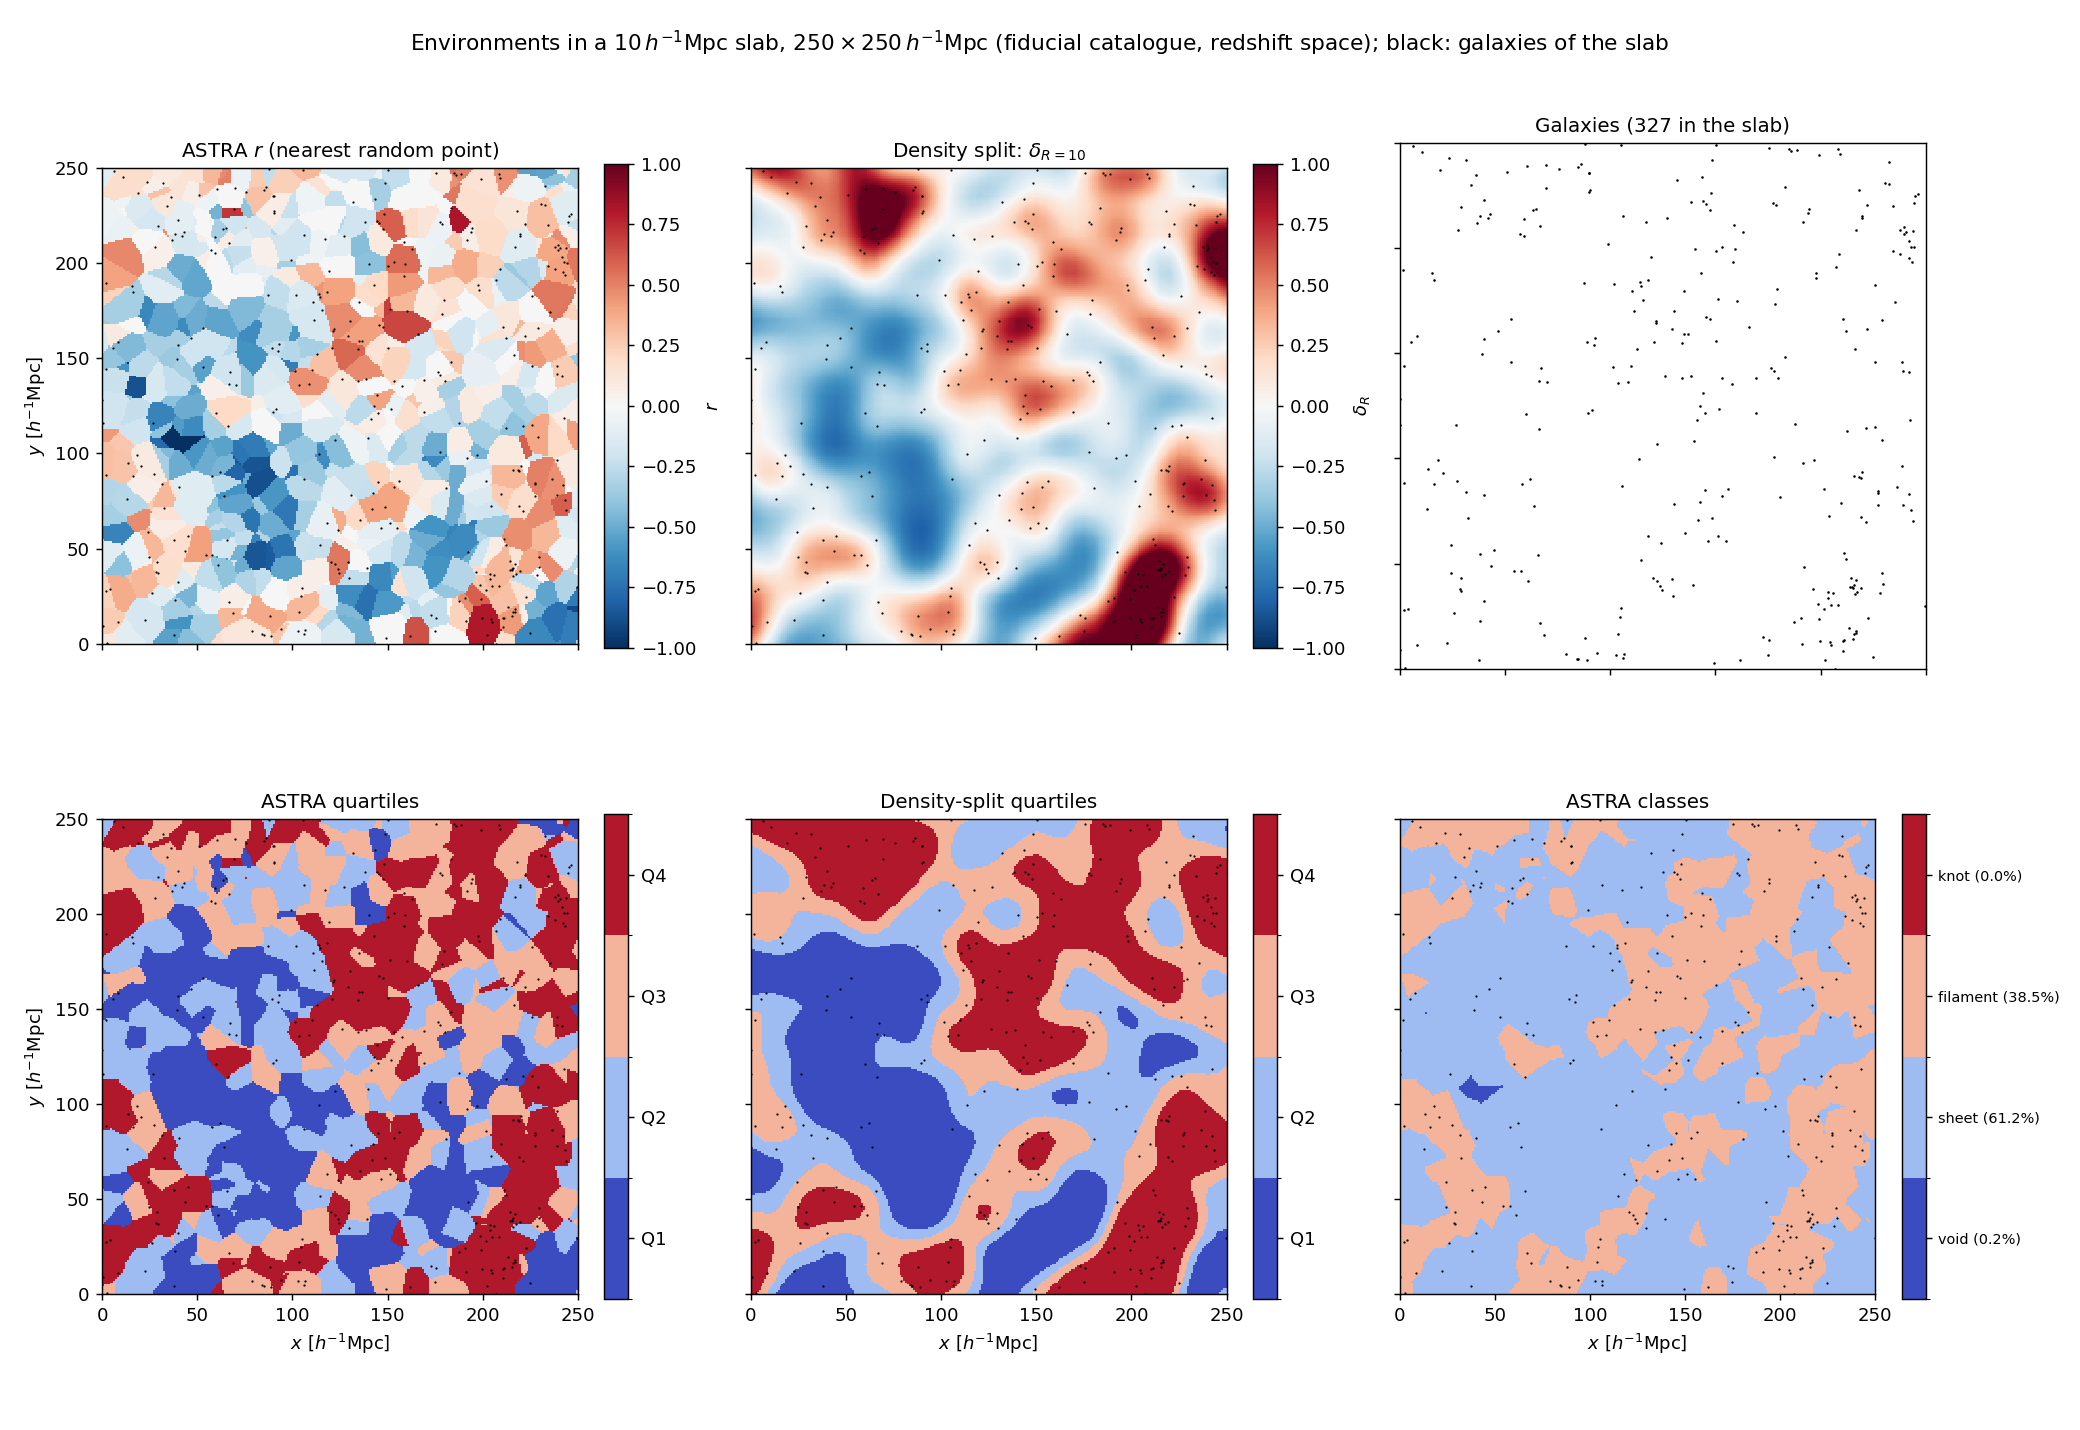
\includegraphics[width=0.95\linewidth]{env_maps.png}
\caption{Les environnements dans une tranche de la simulation : $r$ d'ASTRA et densité lissée du density split (haut), quartiles et classes (bas), galaxies en noir.}
\end{figure}

\end{document}
